% !TEX root = ../thesis-WW.tex

\chapter{Matrix Fisher-Gaussian Distribution} \label{chap:MFG}

The matrix Fisher and Bingham distributions can model large uncertainty for 3D rotations, and have been used in various engineering applications.
However, in practical estimation problems, the attitude is often coupled with other quantities in Euclidean space, such as sensor biases, velocity, position, and landmark locations, etc.
Moreover, the correlation between attitude and these Euclidean quantities are usually very important in estimation problems.
For example, in an attitude filter, the gyroscope bias cannot be directly measured, but it can be corrected because it is correlated with the attitude which can be estimated by direction sensors.
Similarly, in IMU-GNSS integration, the attitude is usually not measured, but it can be corrected by its correlation with position which is directly measured.
The matrix Fisher and Bingham distributions, defined on $\SO{3}$ and $\Sph^3$, cannot deal with the correlation between rotations and random variables in Euclidean space.

Despite the fact that there have been attempts to construct a new probability density function on $\SO{3} \times \mathbb{R}^n$ \cite{darling2016uncertainty,markley2006attitude}, as reviewed in Chapter \ref{section:intro-review-estimation}, there are still motivations to build a new model that
(i) deals with the correlation between attitude and Euclidean random variables not restricted to position,
and (ii) has a closed form maximum likelihood estimation of its parameters for efficient inference.
With such a new model, the matrix Fisher distribution can be generalized to be used in a lot of classic estimation problems where the attitude and other Euclidean quantities must be estimated concurrently.

This chapter introduces a new probability density function on $\SO{3}\times \mathbb{R}^n$, referred to as the matrix Fisher--Gaussian (MFG) distribution.
It is constructed using the conditioning approach which is a generic method of constructing new distributions in directional statistics \cite{pewsey2021recent}.
In particular, a Gaussian distribution with a special structure is conditioned from $\mathbb{R}^9\times \mathbb{R}^n$ onto $\SO{3}\times \mathbb{R}^n$, such that only the \textit{linear} correlation between $\SO{3}$ and $\mathbb{R}^n$ is described by $3n$ parameters.
Due to this geometric construction, the correlation has an immediate geometric interpretation.
And a more desirable result is that the MLE for the parameters of MFG has a closed form approximation, which eliminates the need for a numerical optimization, hence has the potential to be implemented in real time for an estimation algorithm.

Depending on the structure of the Gaussian distribution in $\mathbb{R}^9\times \mathbb{R}^n$ before conditioning, the MFG has two forms, referred to as the MFGI and MFGB respectively.
For MFGI, the rotation in the inertial frame (multiplied on the left) is correlated with $\mathbb{R}^n$; whereas for MFGB the rotation in the body-fixed frame (multiplied on the right) is correlated with $\mathbb{R}^n$.
This highlights the non-commutative nature of $\SO{3}$, and has not been seen in other probability models where the operation for the underlying space is commutative.

Based on the homomorphism between $\SO{3}$ and $\Sph^3$, and the equivalence between matrix Fisher and Bingham distributions, the Bingham--Gaussian (BG) distribution on $\Sph^3\times \mathbb{R}^n$ is also constructed.
As expected, the MFG and BG are also equivalent.

From this chapter, the following notations will be used: $e_i$ represents the $i$-th column of $I_{m\times m}$ for $i=1,\ldots,m$, where $m$ will be clear from the context.

\section{Definition and Construction}

This section gives a formal definition of the matrix Fisher distribution on $\SO{3}\times\mathbb{R}^n$, and its construction by conditioning a Gaussian distribution from $\mathbb{R}^9\times \mathbb{R}^n$ is presented.

\subsection{Definition}

\begin{definition} \label{def:MFG}
	The random elements $(R,x)\in\mathrm{SO}(3)\times\mathbb{R}^n$ follow the matrix Fisher--Gaussian distribution with parameters $\mu\in\mathbb{R}^n$, $\Sigma=\Sigma^T\in\mathbb{R}^{n\times n}$, $U,V\in\mathrm{SO}(3)$, $S=\mathrm{diag}(s_1,s_2,s_3)\in\mathbb{R}^{3\times 3}$ with $s_1 \geq s_2 \geq |s_3| \geq 0$ and $P\in\mathbb{R}^{n\times 3}$, if it has the following density function:
	\begin{align} \label{eqn:MFG-density}
		p(R,x) = \frac{1}{c(S)\sqrt{(2\pi)^n\mathrm{det}({\Sigma}_c)}}\exp\left\{-\tfrac{1}{2}(x-\mu_c)^T\Sigma_c^{-1}(x-\mu_c)\right\} \mathrm{etr}\left\{FR^T\right\},
	\end{align}
	where  $\mu_c\in\mathbb{R}^n$ is given by
	\begin{equation} \label{eqn:MFG-Miuc}
		\mu_c = \mu+P\nu_R.
	\end{equation}
	The expression for $\nu_R$ has two forms, which defines the two variants of MFG, namely MFGI and MFGB:
	\begin{subequations} \label{eqn:MFG-vR}
		\begin{flalign}
			\text{(MFGI)} && \nu_R^B &= (QS-SQ^T)^\vee, && \label{eqn:MFG-vR-MFGI} \\
			\text{(MFGB)} && \nu_R^I &= (SQ-Q^TS)^\vee, && \label{eqn:MFG-vR-MFGB}
		\end{flalign}
	\end{subequations}
	with ${Q}=U^TRV$.
	In addition, $0\prec {\Sigma}_c\in\mathbb{R}^{n\times n}$ is defined as
	\begin{equation} \label{eqn:MFG-Sigmac}
		\Sigma_c = \Sigma-P(\tr{S}I_{3\times 3}-S)P^T,
	\end{equation}
	Also, $F=USV^T\in\mathbb{R}^{3\times 3}$, and $c(S)\in\mathbb{R}$ is the normalizing constant of the corresponding matrix Fisher distribution.
	This distribution is denoted by $\mathcal{MG}(\mu,\Sigma,P,U,S,V)$.
\end{definition}

The probability density function of MFG given by \eqref{eqn:MFG-density} is composed of three terms:
the first one is for normalization; the second term is for $x$ and it has the form as $\mathcal{N}(\mu_c, \Sigma_c)$; the last term is for $R$ and it is identical to the matrix Fisher Distribution. 
From its definition, it is straightforward to see that the marginal distribution of $R$ is a matrix Fisher distribution with parameter $F$, and
the distribution of $x$ conditioned by $R$ is Gaussian with $x|R\sim\mathcal{N}(\mu_c(R), \Sigma_c)$. 

When $P=0$, $x$ and $R$ are independent, and they further satisfy $x\sim\mathcal{N}(\mu,\Sigma)$ and $R\sim\mathcal{M}(F)$.
As such, the attitude-linear correlation is specified by the $3n$ elements of $P$.
More specifically, the correlation between $x$ and $R$ is caused by the fact that the conditional mean $\mu_c(R)$ of $x$ is dependent on $R$. 
When conditioned by $R$, it is shifted by $P\nu_R$ in \eqref{eqn:MFG-Miuc}, where $\nu_R$ in \eqref{eqn:MFG-vR} indicates how $R$ deviates from the mean attitude $UV^T$. 
For example, when $R=UV^T$, or equivalently when $Q=I_{3\times 3}$, we have $\nu_R=0$ and $\mu_c=\mu$.

It should be noted that the MFG must be defined using the proper singular value decomposition $USV^T = F$, not the single parameter $F$.
This is because the principal axes specified by $F$ is not unique for degenerative cases when the diagonal matrix $S$ has repeated values, but MFG must specify the exact principal axis that is correlated with $x\in\mathbb{R}^n$.
The non-uniqueness of pSVD also makes the Definition \ref{def:MFG} not unique, in the sense that the same MFG can be parameterized by different parameters.

More specifically, there are two uniqueness issues associated with the definition of pSVD.
The trivial one is that when $U$ and $V$ undergo simultaneous sign changes of two columns, they are still the left and right proper singular vectors of $F$.
The other issue is more interesting: when $F$ has repeated singular values, the corresponding proper singular vectors in $U$ and $V$ are only unique up to a rotation.
To study how the same MFG can be parameterized differently, it is first shown that MFG can be uniquely parameterized by the intermediate parameters $F$, $\mu_c$ and $\Sigma_c$.

\begin{lemma} \label{lemma:MFG-equivalent-intermediate}
	Two matrix Fisher--Gaussian distributions, namely $\mathcal{MG}(\mu,\allowbreak \Sigma,\allowbreak P,\allowbreak U,\allowbreak S,\allowbreak V)$ and $\mathcal{MG}(\tilde{\mu},\allowbreak \tilde{\Sigma},\allowbreak \tilde{P},\allowbreak \tilde{U},\allowbreak \tilde{S},\allowbreak \tilde{V})$ are equivalent if and only if $F=\tilde{F}$, $\mu_c = \tilde{\mu}_c$ for all $R\in\SO{3}$, and $\Sigma_c = \tilde{\Sigma}_c$.
\end{lemma}

The proof of this lemme requires the a further lemma, which states that a matrix Fisher distribution is uniquely parameterized by its parameter $F$.

\begin{lemma} \label{lemma:MF-equivalent}
	Two matrix Fisher distributions, namely  $\mathcal{M}(F)$ and $\mathcal{M}(\tilde F)$ are equivalent if and only if $F=\tilde{F}$.
\end{lemma}
\begin{proof}
	It is trivial to show $F = \tilde F$ implies $\mathcal{M}(F)=\mathcal{M}(\tilde F)$.
	Next, suppose $\mathcal{M}(F)=\mathcal{M}(\tilde F)$, i.e.,  $\frac{\etr{FR^T}}{c(F)} = \frac{\etr{\tilde{F}R^T}}{c(\tilde{F})}$ for all $R\in\SO{3}$.
	Let $\Delta F = F-\tilde{F}$ and $\Delta c = \log(c(F)/c(\tilde{F}))$, the above equation is equivalent to
	\begin{equation} \label{eqn:MFEquivalent}
		\tr{\Delta FR^T} - \Delta c = 0.  
	\end{equation}
	Substitute $R = I_{3\times3}$, $\expb{\pi\hat{e}_1}$, $\expb{\pi\hat{e}_2}$ and $\expb{\pi\hat{e}_3}$ into \eqref{eqn:MFEquivalent} to obtain
	\begin{align*}
		\Delta F_{11} + \Delta F_{22} + \Delta F_{33} - \Delta c &= 0, \\
		\Delta F_{11} - \Delta F_{22} - \Delta F_{33} - \Delta c &= 0, \\
		-\Delta F_{11} + \Delta F_{22} - \Delta F_{33} - \Delta c &= 0, \\
		-\Delta F_{11} - \Delta F_{22} + \Delta F_{33} - \Delta c &= 0,
	\end{align*}
	which shows $\Delta F_{11} = \Delta F_{22} = \Delta F_{33} = \Delta c = 0$.
	Next, substituting $R = \begin{bmatrix} 0 & 1 & 0 \\ 1 & 0 & 0 \\ 0 & 0 & -1 \end{bmatrix}$ and $\begin{bmatrix} 0 & -1 & 0 \\ 1 & 0 & 0 \\ 0 & 0 & 1 \end{bmatrix}$ into \eqref{eqn:MFEquivalent} yields $\Delta F_{21} = 0$.
	Similarly, other entries of $\Delta F$ can be shown to be zeros. 
	Therefore, $F=\tilde{F}$.
\end{proof}

Next, the proof for Lemma \ref{lemma:MFG-equivalent-intermediate} is as follows.

\begin{proof}[Proof for Proposition \ref{lemma:MFG-equivalent-intermediate}]
	The sufficiency directly follows from \eqref{eqn:MFG-density} since the density function is determined by $F$, $\mu_c$ and $\Sigma_c$.
	Next we show the necessity.
	Let $p$ and $\tilde p$ be the density functions for the two sets of parameters respectively.
	Suppose $p(x,R) = \tilde p(x, R)$  for all $x\in\mathbb{R}^n$ and $R\in\SO{3}$.
	Since $\SO{3}$ is compact, and $\mu_c$ is continuous in $R$ as seen from \eqref{eqn:MFG-Miuc}, $\norm{\mu_c}$ has an upper bound.
	Therefore,
	\begin{equation*}
		\lim\limits_{\norm{x}\to\infty} p(x,R) = \frac{\etr{FR^T}}{c(F)\sqrt{(2\pi)^n\mathrm{det}({\Sigma}_c)}}.
	\end{equation*}
	Because $p(x,R) = \tilde p(x,R)$ for all $x\in\mathbb{R}^n$, the above equation implies $\frac{\etr{FR^T}}{c(F)\sqrt{(2\pi)^n\det(\Sigma_c)}} = \frac{\etr{\tilde{F}R^T}}{c(\tilde{F})\sqrt{(2\pi)^n\det(\tilde{\Sigma}_c)}}$, and by following the same argument in Lemma \ref{lemma:MF-equivalent}, $F=\tilde{F}$.
	
	Next, since $F=\tilde{F}$ and $p(x,R) = \tilde p(x,R)$, we have $(x-\mu_c)^T\Sigma_c^{-1}(x-\mu_c) = (x-\tilde{\mu}_c)^T \tilde{\Sigma}_c^{-1} \allowbreak (x-\tilde{\mu}_c)$ for all $x\in\mathbb{R}^n$ and $R\in\SO{3}$.
	Substituting $x = \mu_c$ yields $\mu_c = \tilde{\mu}_c$ for all $R\in\SO{3}$, since $\tilde{\Sigma}_c$ is positive definite.
	Also, substituting $x = \mu_c+e_i$ shows $(\Sigma_c^{-1})_{ii} = (\tilde{\Sigma}_c^{-1})_{ii}$, and similarly, substituting $x = \mu_c+e_i+e_j$ for $i \neq j$ yields $(\Sigma_c^{-1})_{ij} = (\tilde{\Sigma}_c^{-1})_{ij}$ since $\Sigma_c^{-1}$ and $\tilde{\Sigma}_c^{-1}$ are symmetric.
	Therefore $\Sigma_c = \tilde{\Sigma}_c$.
\end{proof}

Using Lemma \ref{lemma:MFG-equivalent-intermediate}, it can be shown that the same MFG can be parameterized by simultaneously reversing the signs of any two columns of $U$, $V$, and $P$.
This resolves the non-uniqueness of pSVD caused by simultaneous sign changes.
\begin{theorem}
	Let $L = \expb{\pi\hat{e}_i}$, for $i=1,2,\text{ or }3$, then $\mathcal{MG}(\mu,\allowbreak \Sigma,\allowbreak P,\allowbreak U,\allowbreak S,\allowbreak V)$ and $\mathcal{MG}(\mu,\allowbreak \Sigma,\allowbreak PL,\allowbreak UL,\allowbreak S,\allowbreak VL)$ are equivalent.
\end{theorem}
\begin{proof}
	Let $F$, $\mu_c$, $\Sigma_c$ and $\tilde{F}$, $\tilde{\mu}_c$, $\tilde{\Sigma}_c$ be the intermediate parameters of the two MFGs respectively, as stated in Lemma \ref{lemma:MFG-equivalent-intermediate}.
	Then it is clear that
	\begin{align*}
		\tilde{F} &= ULSL^TV^T = USV^T = F, \\
		\tilde{\Sigma}_c &= \Sigma-PL(\tr{S}I_{3\times 3}-S)L^TP^T = \Sigma_c,
	\end{align*}
	and for all $R\in\SO{3}$,
	\begin{align*}
		\tilde{\mu}_c &= \mu + PL(SL^TU^TRVL - L^TV^TR^TUDS)^\vee \\
		&= \mu + P(LSL^TU^TRV - V^TR^TULSL^T)^\vee = \mu_c.
	\end{align*}
	Therefore by Lemma \ref{lemma:MFG-equivalent-intermediate}, the two MFGs are equivalent.
\end{proof}

Next, to deal with the non-uniqueness issue caused by repeated singular values, the space of eigen vectors must be analyzed in detail depending on the multiplicity of $S$.
In Appendix \ref{app:MFG-unique}, a complete characterization of how the MFG can be parameterized differently if $S$ has repeated values is given.

\subsection{Construction}

The construction of MFG is motivated by \cite{mardia1978model}, where a distribution on the cylinder is constructed by conditioning a three-dimensional Gaussian distribution from $\mathbb{R}^3$ into $\mathbb{S}^1 \times \mathbb{R}^1$.
However, in \cite{mardia1978model} two parameters are used to quantify the angular-linear correlation, despite both of the angular part $\mathbb{S}^1$ and the linear part $\mathbb{R}^1$ are one-dimensional.
This is because the correlation is formulated between the ambient space of $\mathbb{S}^1$, namely $\mathbb{R}^2$, and $\mathbb{R}^1$.

\begin{figure}
	\centering
	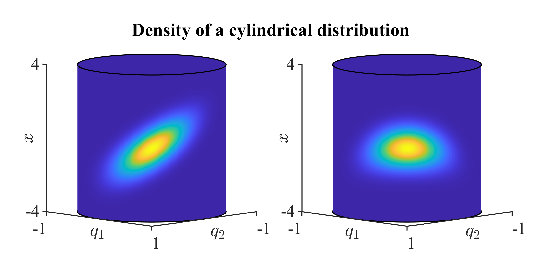
\includegraphics[scale=1.4]{figures/MFG-angular-linear-correlation}
	\caption{The illustration of the cylindrical distribution with the mean angle $\pi/4$~\cite{mardia1978model}.
		In the left figure, the correlation between the linear variable $x\in\mathbb{R}$ and the angular variable $q=(q_1,q_2)\in\Sph^1$ is only nonzero along the tangent direction of $\mathbb{S}^1$ at $\pi/4$, and the distribution of $q$ conditioned by $x$ varies as $x$ is altered, and vice versa. 
		However in the right figure,  the correlation is specified along the radial direction of $\Sph^1$, and there is no clear correlation between $x$ and $q$.
		These illustrate the correlation along the tangent direction captures what we expect as a \textit{linear} correlation between two random variables.
		\label{fig:MFG-angular-linear-correlation}}
\end{figure}

In general, the correlation between two random variables describes how one random variable is linearly varied from its mean, when the other random variable is perturbed from its own mean. 
As such, we wish that the correlation between $\Sph^1$ and $\mathbb{R}^1$ is described by a single parameter. 
The key observation is that the unit-vector in $\Sph^1$ cannot be varied from the mean exclusively along the radial direction due to the unit-length constraint. 
Further, when it is rotated, the variation along the radial direction is constrained by the variation along the tangential direction. 
Thus, the correlation between $\Sph^1$ and $\mathbb{R}^1$ can be described by the correlation between the linear variable and the \textit{tangential} direction of the angular variable at the mean angle.
This is illustrated in Fig. \ref{fig:MFG-angular-linear-correlation}.

Similarly, if the correlation between $R\in\SO{3}$ and $x\in\mathbb{R}^n$ is defined as in~\cite{mardia1978model}, it needs $9n$ parameters. 
Instead, the ambient space of $\SO{3}$, namely $\mathbb{R}^{3\times 3}$, is decomposed into two parts, namely the tangent space at the mean attitude and its orthogonal complement.
The correlation with linear variables along the orthogonal complement is set to zero, thereby reducing the number of free parameters into $3n$.
More specifically, a Gaussian distribution is formulated on $\mathbb{R}^9\times\mathbb{R}^n$ such that the correlation along the orthogonal complement to the tangent space at the mean attitude is annihilated before conditioning onto $\SO{3}\times\mathbb{R}^n$.

The difference between MFGI and MFGB comes from how $\SO{3}$ is embedded into $\mathbb{R}^9$.
For MFGI, the embedding is $R\mapsto \mathrm{vec}(R^T)$, i.e., the rows of $R$ is concatenated into a vector;
where as for MFGB, the embedding is $R\mapsto \mathrm{vec}(R)$, i.e., the columns of $R$ is concatenated into a vector.
The construction is summarized into the following theorem.
\begin{theorem} \label{thm:MFG-construction}
	Consider the parameters $(\mu,\allowbreak \Sigma,\allowbreak V,\allowbreak S,\allowbreak U,\allowbreak P)$ satisfying the conditions in Definition \ref{def:MFG}.
	Let $M = UV^T$, $K_I = VSV^T$, $K_B = USU^T$.
	Also, let $\mu_I = \mathrm{vec}(M^T)$, $\Sigma_I^{-1} = I_{3\times 3}\otimes K_I$; and $\mu_B = \mathrm{vec}(M)$, $\Sigma_B^{-1} = I_{3\times 3}\otimes K_B$, where $\otimes$ denotes Kronecker product.
	
	Also let $t_{Ii} = \mathrm{vec}\big[(M\widehat{Ve_i})^T\big]$ for $i\in\{1,2,3\}$ be the basis for the tangent space of $\SO{3}$ at $M$ embedded in $\mathbb{R}^9$, and $t_{Bi} = \mathrm{vec}\big[M\widehat{Ve_i}\big]$.
	Define $T_I = [t_{I1},\cdots,t_{I9}] \in \mathbb{R}^{9\times 9}$ such that $T_I\in\SO{9}$, and $P_I = [P,0_{n\times 6}]T_I$.
	Similarly, define $T_B = [t_{B1},\cdots,t_{B9}] \in \mathbb{R}^{9\times 9}$ such that $T_B\in\SO{9}$, and $P_B = [P,0_{n\times 6}]T_B$.
	
	Suppose $\big(\mathrm{vec}(R^T),x\big)\in\mathbb{R}^{9+n}$ follows the Gaussian distribution
	\begin{align} \label{eqn:MFG-construct-condition-MFGI}
		\begin{bmatrix} \mathrm{vec}(R^T) \\ x \end{bmatrix} 
		\sim \mathcal{N}\! \left(
		\begin{bmatrix} \mu_I \\ \mu \end{bmatrix},
		\begin{bmatrix}
			\Sigma_I & P_I^T \\
			P_I & \Sigma
		\end{bmatrix} \right),
	\end{align}
	then the density for $(R,x)$ is \eqref{eqn:MFG-density} with $\nu_R$ defined in \eqref{eqn:MFG-vR-MFGI} when restricted to $R\in\SO{3}$.
	Suppose instead $\big(\mathrm{vec}(R),x\big)\in\mathbb{R}^{9+n}$ follows the Gaussian distribution
	\begin{align} \label{eqn:MFG-construct-condition-MFGB}
		\begin{bmatrix} \mathrm{vec}(R) \\ x \end{bmatrix} 
		\sim \mathcal{N}\! \left(
		\begin{bmatrix} \mu_B \\ \mu \end{bmatrix},
		\begin{bmatrix}
			\Sigma_B & P_B^T \\
			P_B & \Sigma
		\end{bmatrix} \right),
	\end{align}
	then the density for $(R,x)$ is \eqref{eqn:MFG-density} with $\nu_R$ defined in \eqref{eqn:MFG-vR-MFGB} when restricted to $R\in\SO{3}$.
\end{theorem}
\begin{proof}
	First consider \eqref{eqn:MFG-construct-condition-MFGI}.
	The joint density of $\big(\mathrm{vec}(R^T),x\big)$ can be written in the form of a conditional-marginal density as
	\begin{align}
		p\big(\mathrm{vec}(R^T),x\big) \propto &\expb{-\tfrac{1}{2}(x-\mu'_c)^T (\Sigma'_c)^{-1} (x-\mu'_c)} \nonumber \\
		\cdot &\expb{-\tfrac{1}{2}(\mathrm{vec}(R^T)-{\mu}_I)^T \Sigma_I^{-1} (\mathrm{vec}(R^T)-{\mu}_I)},
	\end{align}
	$\mu'_c = \mu+P_I\Sigma_I^{-1}\big(\mathrm{vec}(R^T)-\mu_I\big) \in \mathbb{R}^n$, and $\Sigma'_c = \Sigma-P_I\Sigma_I^{-1}P_I^T \in \mathbb{R}^{n\times n}$.
	The second exponential term has been proved in Theorem \ref{thm:MF-construction} to be proportional to $\etr{FR^T}$, where $F=USV^T$.
	So it remains to check for all $R\in\SO{3}$, $\mu'_c = \mu_c$ in \eqref{eqn:MFG-Miuc}, and $\Sigma'_c = \Sigma_c$ in \eqref{eqn:MFG-Sigmac}.
	
	For $\Sigma'_c$, it can be shown that
	\begin{equation*}
		P_I\Sigma_I^{-1}P_I^T = P[t_{I1},t_{I2},t_{I2}]^T\Sigma_I^{-1}[t_{I1},t_{I2},t_{I2}]P^T 
		\triangleq P \tilde{\Sigma}_I^{-1} P^T,
	\end{equation*}
	for some $\tilde{\Sigma}_I^{-1} \in \mathbb{R}^{3\times 3}$.
	Let $t_{Ii}\in\mathbb{R}^9$ be equally split into three vectors $\{t_{Ii1},t_{Ii2},t_{Ii3}\}$, then the $(i,j)$-th entry of $\tilde{\Sigma}_I^{-1}$ can be written as
	\begin{align*}
		(\tilde{\Sigma}_I^{-1})_{ij} &= \sum_{k=1}^3t_{Iik}^T K_I t_{Ijk} = \tr{[t_{Ii1},t_{Ii2},t_{Ii3}]^T K_I [t_{Ij1},t_{Ij2},t_{Ij3}]} \nonumber \\
		&= \tr{ M \widehat{Ve_i} K_I \widehat{Ve_j}^T M^T }
		= \tr{S\hat{e}_j^T\hat{e}_i},
	\end{align*}
	which implies $\tilde{\Sigma}_I^{-1} = \tr{S}I_{3 \times 3}-S$, so $\Sigma'_c = \Sigma_c$ in \eqref{eqn:MFG-Sigmac}.
	Next, the second part of $\mu'_c$ is
	\begin{equation*}
		P_I\Sigma_I^{-1}\big(\mathrm{vec}(R^T)-\mu_I\big) = P[t_{I1},t_{I2},t_{I2}]^T\Sigma_I^{-1}\mathrm{vec}(R^T-M^T),
	\end{equation*}
	where the $i$-th element of $[t_{I1},t_{I2},t_{I2}]^T\Sigma_I^{-1}\mathrm{vec}(R^T-M^T)$ can be calculated as
	\begin{gather*}
		t_{Ii}^T\Sigma_I^{-1} \mathrm{vec}(R^T-M^T)
		= \tr{M\widehat{Ve_i}K(R^T-M^T)} = \tr{SQ^T\hat{e}_i - S\hat{e}_i} = e_i^T(QS-SQ^T)^\vee, 
	\end{gather*}
	and ${Q} = U^TRV$.
	This shows $\mu'_c = \mu_c$ in \eqref{eqn:MFG-Miuc} for all $R\in\SO{3}$, and finishes the proof of the case \eqref{eqn:MFG-construct-condition-MFGI} for MFGI.
	The proof of \eqref{eqn:MFG-construct-condition-MFGB} for MFGB follows exactly the same steps, and is omitted for brevity.
\end{proof}

In Theorem \ref{thm:MFG-construction}, the covariance for MFGI between $\mathrm{vec}(R^T)$ and $x$ is $P_I =[ P, 0_{n\times 6}]T_I$, i.e., it is non-zero only along $\{t_{I1}, t_{I2}, t_{I3}\}$, which is a basis for the tangent space of $\SO{3}$ at the mean attitude $M=UV^T$.
It is similar for MFGB where the correlation between $\mathrm{vec}(R)$ and $x$ is only non-zero along $\{t_{B1}, t_{B2}, t_{B3}\}$.
The basis of the tangent space is chosen as the principal axes of the matrix Fisher part, so that the correlation $P$ is expressed with respect to the principal axes, which simplifies the corresponding mathematical analysis and provides geometric interpretations.
Also, there are only $3n$ parameters required to quantify the linear correlation between the three-dimensional attitude and the $n$-dimensional linear variable, instead of $9n$.

\begin{figure}
	\centering
	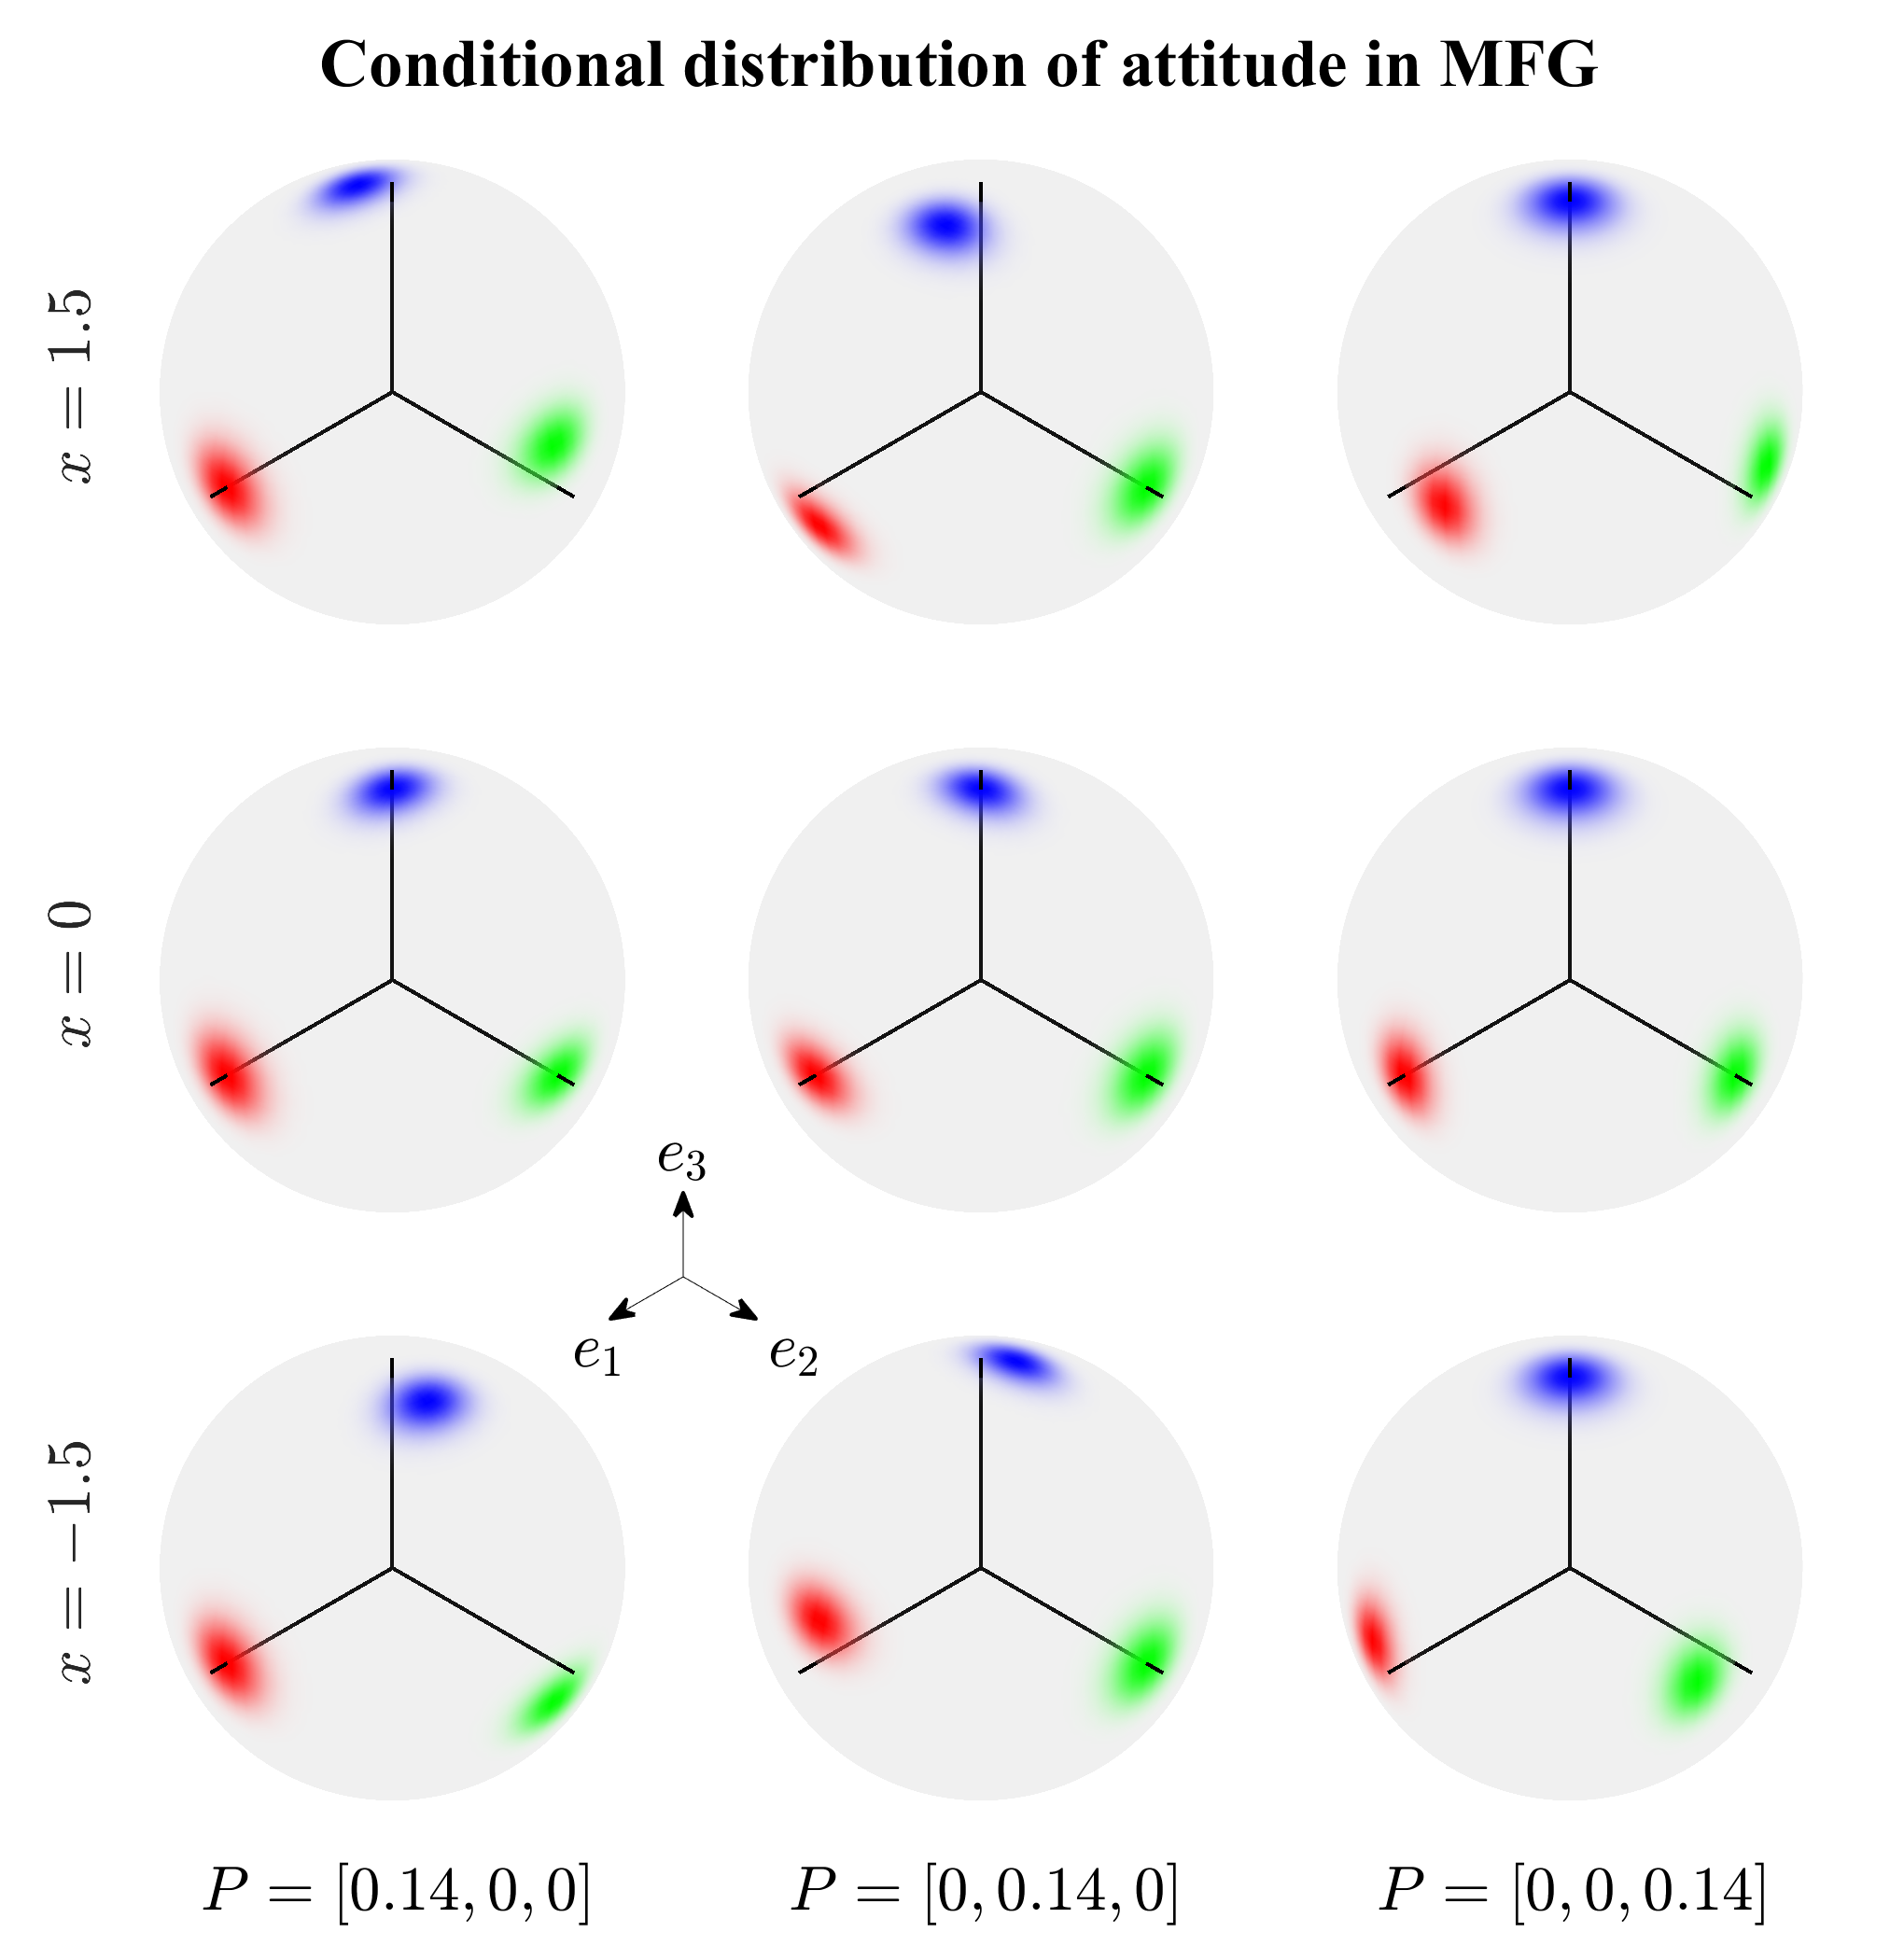
\includegraphics[scale=1.4]{figures/MFG-correlation}
	\caption{Visualization of the attitude-linear correlation (MFGB) for $(R,x)\in\SO{3}\times\mathbb{R}^1$: the density for $R$ conditioned on $x$ is illustrated on the unit-sphere for three correlation matrices $P$. 
		More specifically, the marginal distribution for each column of $R$ is shown on the unit sphere as red, green and blue shades. 
		The parameters are $n=1$, $\mu=0$, $\Sigma=1$, $U=V=I_{3\times3}$, $S=10I_{3\times3}$.
		For each  $P$, three conditioning values of $x$ are considered. 
		The first column is for $P=[0.14,0,0]$.
		When $x$ is increased from $-1.5$ to $1.5$, the conditional distribution for $R$ is rotated about the $e_1$ axis. 
		Similarly, in the second column for $P=[0,0.14,0]$, the variation of $x$ is correlated with rotating the distribution of $R$ along the $e_2$ axis.
		The third column shows rotations about $e_3$ due to the correlation. \label{fig:MFG-correlation}}
\end{figure}

This construction of MFG leads to a clear geometric interpretation of the correlation parameter $P$:
if $P_{ij} > 0$, as $x_i$ becomes increased, the distribution of $R$ conditioned on $x$ rotates about the $j$-th principal axis of the matrix Fisher part, and vice versa.
See Fig. \ref{fig:MFG-correlation} for a simple example exhibited for MFGB.

\subsection{Distinction Between MFGI and MFGB} \label{section:MFG-MFGI-MFGB}

At first glance, it appears that the MFGI and MFGB are very similar, as the difference is caused by the single term $\nu_R$ in \eqref{eqn:MFG-vR}.
In this subsection, the implications of the two definitions of $\nu_R$ and its role in formulating the angular--linear correlation are discussed.

More specifically, the difference is studied by examining $R|x$, the attitude distribution of $R$ conditioned by the linear random variable $x$, when $(R,x)$ is close to the mean $(M=UV^T, \mu)$.
For simplicity, assume the dimension of $x$ is $n=1$, and let $(R,x) \sim \mathcal{MG}(\mu,\allowbreak \sigma^2,\allowbreak P,\allowbreak U,\allowbreak S,\allowbreak V)$.
For both definitions, the density function can be written as
\begin{align*}
	p(R|x) \propto \etr{SQ^T} \exp\left\{ \frac{x-\mu}{\sigma_c^2}P\nu_R - \frac{(P\nu_R)^2}{2\sigma_c^2} \right\},
\end{align*}
where $Q = U^TRV$, and $\sigma_c^2 = \sigma^2 - P(\tr{S}I_{3\times 3}-S)P^T\in\mathbb{R}$.
As $R\rightarrow M$, $Q\rightarrow I_{3\times 3}$ and $\nu_R \rightarrow 0$.
Therefore, when the attitude is close to the mean attitude, the second order term $(P\nu_R)^2$ may be omitted.

For MFGB, $P\nu_R = \tr{\widehat{P^T} Q^TS}$ from \eqref{eqn:SO3-trhatxA} and \eqref{eqn:MFG-vR-MFGB}.
Thus,
\begin{align*} 
	p(R|x) \propto \etr{SQ^T} \etr{\frac{x-\mu}{\sigma_c^2} \widehat{P^T} Q^TS} = \etr{\left(I_{3\times 3} + \hat{\upsilon}(x)\right) Q^TS},
\end{align*}
where $\upsilon(x) \triangleq (x-\mu)/\sigma_c^2 P^T \in \mathbb{R}^{3\times 1}$.
Note that $\exp(\hat\upsilon(x))=I_{3\times 3} + \hat\upsilon(x) + O(\|\upsilon(x)\|^2)$.
Therefore, when $x$ is also close to $\mu$, it can be rewritten as
\begin{align*}
	p(R|x) &\approx \etr{USV^T\exp(\widehat{V\upsilon}(x))R^T}.
\end{align*}
In short, when $(R,x)$ follows MFGB, the conditional distribution $R|x$ follows the matrix Fisher distribution with
\begin{align} \label{eqn:MFG-p(R|x)-MFGB}
	(R|x)\big|_{\text{MFGB}} \approx \mathcal{M}(USV^T\exp(\widehat{V\upsilon}(x))) 
\end{align}
near the mean value $(M,\mu)$. 
Similarly, $R|x$ of MFGI can be approximated by
\begin{align} \label{eqn:MFG-p(R|x)-MFGI}
	(R|x)\big|_\text{MFGI} \approx \mathcal{M}(\exp(\widehat{U\upsilon}(x))USV^T).
\end{align}

Now we compare \eqref{eqn:MFG-p(R|x)-MFGB} and \eqref{eqn:MFG-p(R|x)-MFGI}.
When $x=\mu$, they are identical, and $R|x \sim \mathcal{M}(USV^T)$. 
Further when $x\neq \mu$, they have the same mean attitude given by $U\exp(\hat{\upsilon}(x))V^T$.
The difference between \eqref{eqn:MFG-p(R|x)-MFGB} and \eqref{eqn:MFG-p(R|x)-MFGI} is caused by how the principal axes of rotations are changed as $x$ is varied. 
For \eqref{eqn:MFG-p(R|x)-MFGB}, as $U$ is fixed, the principal axes remain unchanged with respect to $x$ when perceived from the inertial frame.
However, they rotate about $V\upsilon(x)$ when observed in the body-fixed frame, as $V$ is changed into $\exp(-\widehat{V\upsilon}(x))V$.
Also, \eqref{eqn:MFG-p(R|x)-MFGB} indicates $R|x$ has the same density as $R\exp(\widehat{V\upsilon}(x))$, i.e., the rotation is applied on the right.
Therefore, the correlation term $\upsilon(x)$ causes the attitude distribution to be rotated about the axis $V\upsilon(x)$ resolved in the body-fixed frame.
For example, suppose that the distribution is represented by a set of sample attitudes $\{R_i\}_{i=1}^N$. 
Then, each sample attitude $R_i$ has a distinct axis of rotation given by $R_i V\upsilon(x)$ in the inertial frame.

\begin{figure}
	\centering
	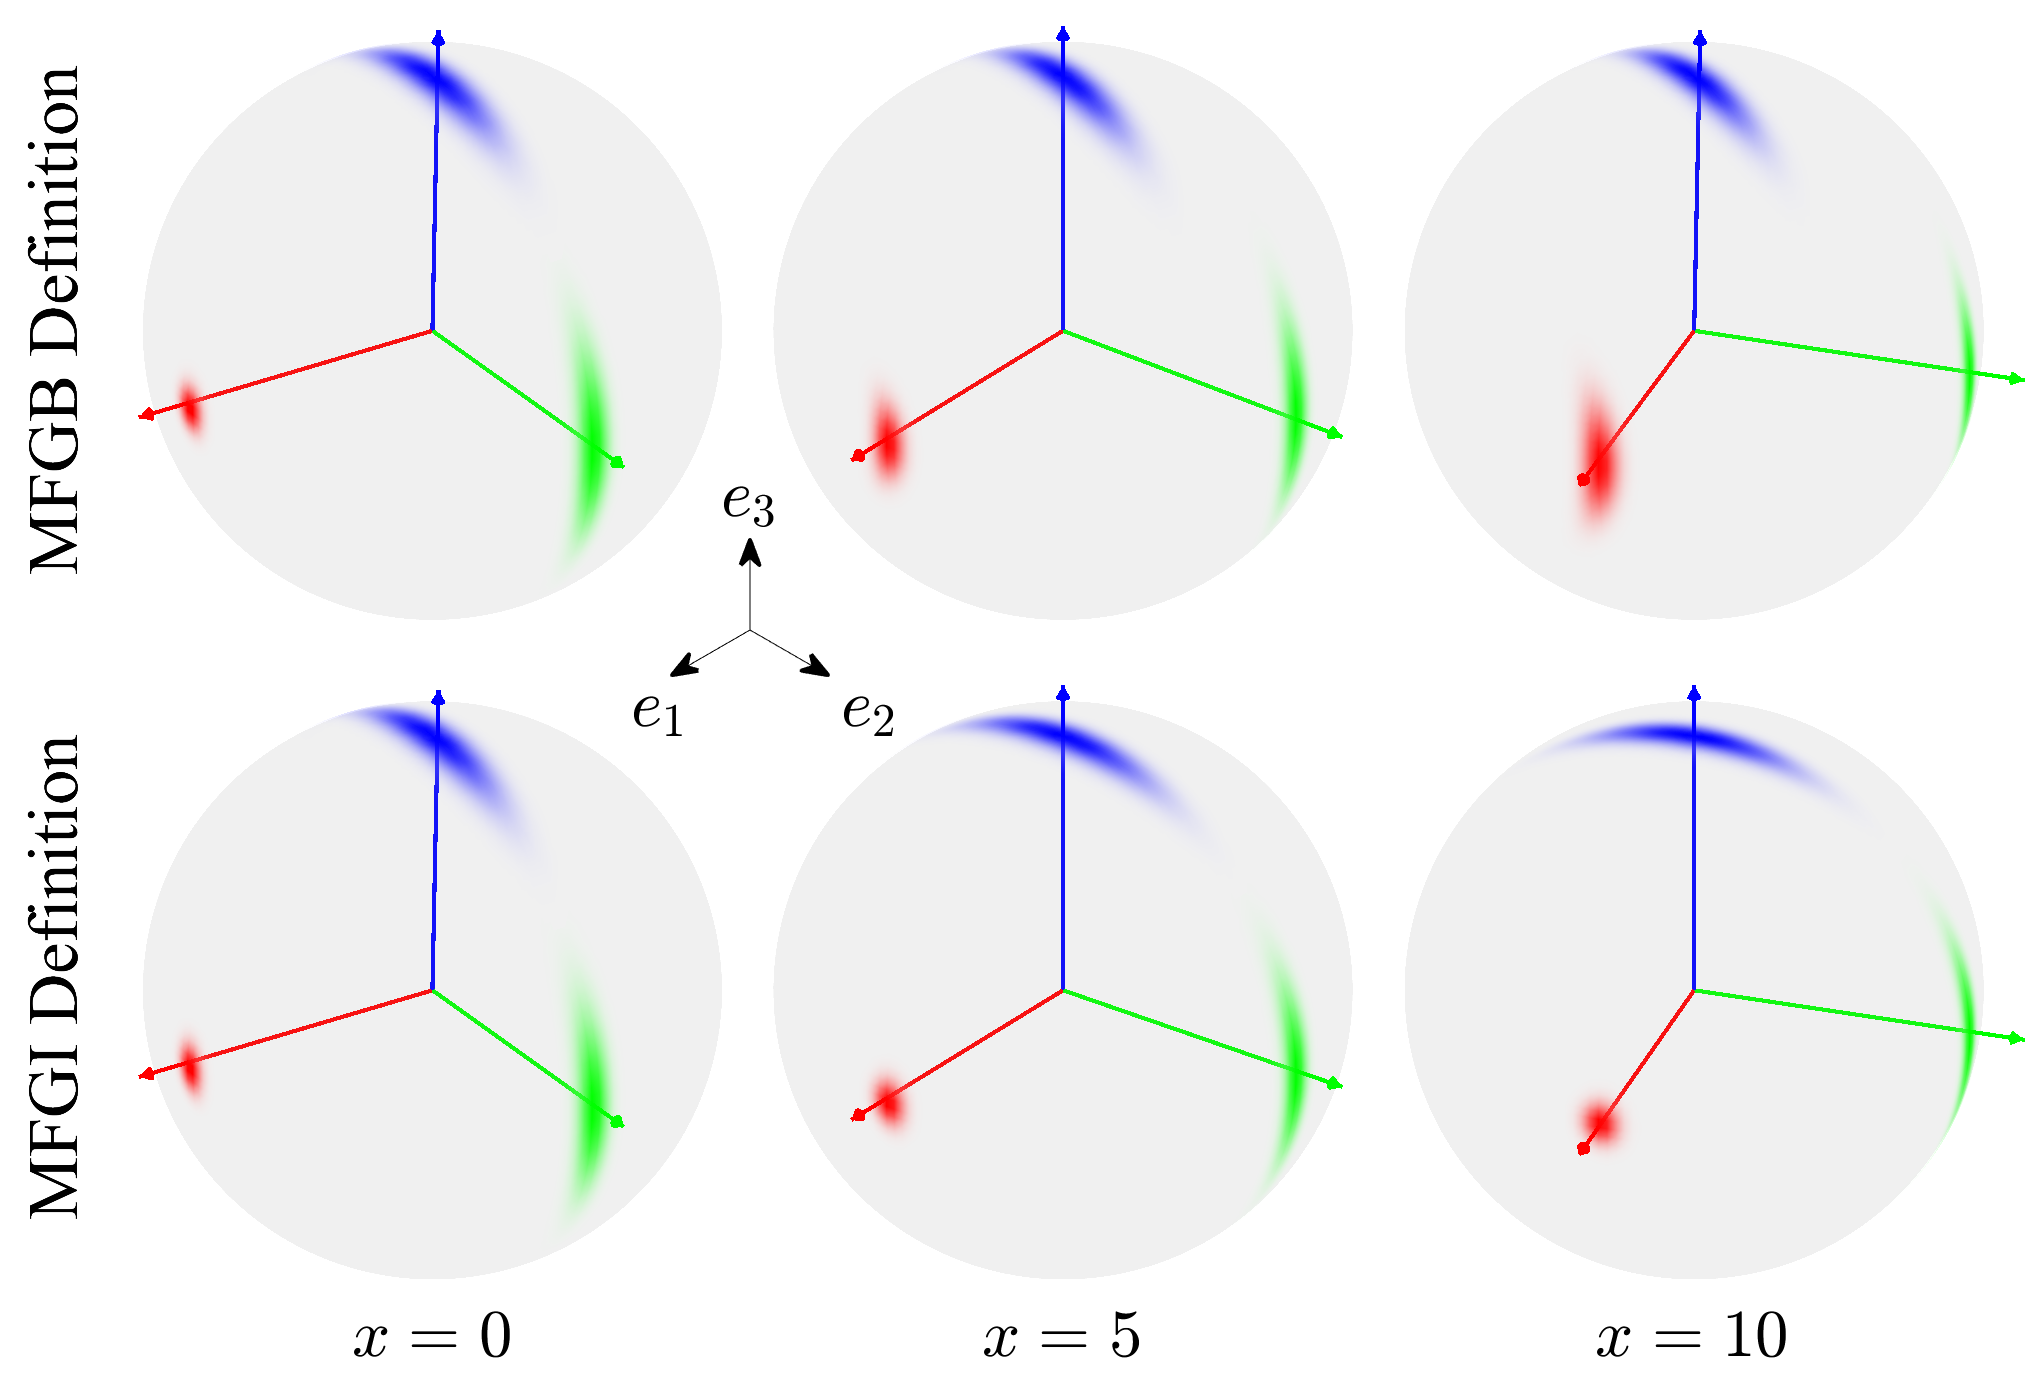
\includegraphics[scale=1.4]{figures/MFG-MFGI-MFGB}
	\caption{Difference between MFGB (top row) and MFGI (bottom row).
		The conditional density of $R|x$ is illustrated on the unit sphere for varying $x$, with the red, green, and blue arrows representing the first, second, and third columns of the mean attitude, respectively.
		Parameters are chosen as $n=1$, $\mu=0$, $\Sigma=1$, $P = [0,0,0.069]$, $U=V=I_{3\times 3}$, $S = \diag(100,3,3)$.
		For both of MFGB and MFBI, the mean attitude of $R|x$ rotates identically about the third inertial axis.
		For MFGI (bottom row), the attitude distribution rotates in the same way as the mean attitude. 
		But for MFGB (top row), it is as if each sample attitude rotates about its own third body-fixed axis. 
		As a result, the distribution of the third axis (blue shade) remains unchanged in the inertial frame. \label{fig:MFG-MFGI-MFGB}}
\end{figure}

On the other hand, in \eqref{eqn:MFG-p(R|x)-MFGI}, the principal axes represented in the inertial frame are rotated, as $U$ is changed into $\exp(\widehat{U\upsilon}(x))U$. 
But, when observed from the body-fixed frame, they remain unchanged. 
Also, \eqref{eqn:MFG-p(R|x)-MFGI} implies $R|x$ has the same density as $\exp(\widehat{U\upsilon}(x))R$, i.e., the rotation is applied on the left. 
This means the correlation term $\upsilon(x)$ causes the attitude distribution to be rotated about the axis $U\upsilon(x)$ resolved in the inertial frame, which is identical for all sample attitudes.

This distinction motivates the naming convention for the two definitions: for MFGB, the correlation causes the attitude distribution to be rotated about the body-fixed frame (multiplied on the right); for MFGI, it causes the distribution to be rotated about the inertial frame (multiplied on the left).
These are illustrated in Fig. \ref{fig:MFG-MFGI-MFGB}.

Finally, when the attitude uncertainty is isotropic, i.e., when $S=sI_{3\times 3}$ for $s \geq 0$, MFGB is identical to MFGI.
As such, the difference between MFGB and MFGI becomes more significant as the attitude distribution is more non-isotropic.

\section{Bingham--Gaussian Distribution}

Before diving into more properties of the MFG, this section first introduces the Bingham--Gaussian (BG) defined on $\Sph^3\times \mathbb{R}^n$ which is equivalent to MFG.
The BG is naturally constructed by transforming MFG use the Lie group homomorphism \eqref{eqn:SO3-Sph3} between $\SO{3}$ and $\Sph^3$.
Due to the prevalence of Bingham distribution in recent literature, the BG can serve as a more accessible model to those who are more familiar with Bingham distribution.

\begin{definition}
	Random elements $(q,x)\in\Sph^3\times\mathbb{R}^n$ follow Bingham-Gaussian distribution with parameters $M\in\SO{4}$, $Z = \diag(0,z_1,z_2,z_3)$ where $0\geq z_1 \geq z_3 \geq z_3$, $\mu\in\mathbb{R}^n$, $\Sigma=\Sigma^T\in\mathbb{R}^{n\times n}$, and $P\in\mathbb{R}^{n\times 3}$, if they have the following density function:
	\begin{align} \label{eqn:BG-density}
		&f(q,x) = \frac{1}{c(Z)\sqrt{(2\pi)^n\det(\Sigma_c)}} \expb{ -\tfrac{1}{2}(x-\mu_c)^T \Sigma_c^{-1} (x-\mu_c) } \expb{q^TMZM^Tq} ,
	\end{align}
	where $c(Z)$ is the normalizing constant for the corresponding Bingham distribution, and $\Sigma_c\in\mathbb{R}^{n\times n}$ satisfying $\Sigma_c = \Sigma_c^T \succ 0$ is given by
	\begin{align}
		\Sigma_c = \Sigma + \frac{1}{2}P\diag(z_1,z_2,z_3)P^T.
	\end{align}
	Depending on the choice of $\mu_c\in\mathbb{R}^n$, there are two formulations of BG. 
	For BGI, $\mu_c\in\mathbb{R}^n$ is given by
	\begin{align} \label{eqn:BG-vq-BGI}
		\mu_c = \mu + P\begin{bmatrix} (z_2-z_3)p_2p_3 - z_1p_0p_1 \\ (z_3-z_1)p_1p_3 - z_2p_0p_2 \\ (z_1-z_2)p_1p_2 - z_3p_0p_3 \end{bmatrix} \triangleq \mu + P\nu_q^I,
	\end{align}
	or, for BGB, $\mu_c$
	\begin{align} \label{eqn:BG-vq-BGB}
		\mu_c = \mu + P\begin{bmatrix} (z_3-z_2)p_2p_3 - z_1p_0p_1 \\ (z_1-z_3)p_1p_3 - z_2p_0p_2 \\ (z_2-z_1)p_1p_2 - z_3p_0p_3 \end{bmatrix} \triangleq \mu + P\nu_q^B,
	\end{align}
	with $p = [p_0, p_1, p_2, p_3]^T \triangleq M^Tq$.
	This distribution is denoted by $\mathcal{BG}(M,Z,\mu,\Sigma,P)$.
\end{definition}

BG is antipodally symmetric in $\Sph^3$, i.e., for any $(q,x)\in\Sph^3\times\mathbb{R}^n$, $f(q,x) = f(-q,x)$.
Similar with MFG, the density \eqref{eqn:BG-density} has three terms:
the first one is for normalization; the second term is for $x$ and it has the form as $\mathcal{N}(\mu_c, \Sigma_c)$; the last term is for $q$ and it is identical to the Bingham distribution.
The marginal distribution of $q$ is a Bingham distribution with parameter $MZM^T$, and the distribution of $x$ conditioned by $q$ is Gaussian with $x|q\sim\mathcal{N}(\mu_c(q), \Sigma_c)$.
Also, the correlation between $q$ and $x$ is represented by the $(3n)$-element matrix $P$.
The vector $\nu_q\in\mathbb{R}^3$ indicates the deviation of $q$ from the mode $m_0$, i.e., if $q=m_0$, then $p = [1,0,0,0]^T$ and hence $\nu_q = 0$.
The two expressions for $\nu_q$ again have the same interpretations as MFG:
If \eqref{eqn:BG-vq-BGI} is used, $x$ is correlated with rotations along the principal axes resolved in the inertial frame (BGI);
if \eqref{eqn:BG-vq-BGB} is used, the rotations are resolved in the body-fixed frame (BGB) of each $q\in\Sph^3$.

The Bingham-Gaussian distribution is constructed by transforming the matrix Fisher-Gaussian distribution using the homomorphism $\varphi: \Sph^3\to\SO{3}$ given in \eqref{eqn:SO3-Sph3}.
\begin{theorem} \label{thm:BG-MFG}
	Let $(M,Z,\mu,\Sigma,P)$ be the parameters of a Bingham-Gaussian distribution.
	Define $S = \diag(s_1,s_2,s_3)$ as $s_1 = \tfrac{1}{4}(z_1-z_2-z_3)$, $s_2 = \tfrac{1}{4}(z_2-z_1-z_3)$, and $s_3 = \tfrac{1}{4}(z_3-z_1-z_2)$.
	Let $M = [u]_L[v^{-1}]_R$ be its isoclinic decomposition.
	Define $U = \varphi(u)$ and $V = \varphi(v)$.
	Then $(q,x)\sim\mathcal{BG}(M,Z,\mu,\Sigma,P)$ if and only if $(\varphi(q),x)\sim\mathcal{MG}(U,S,V,\mu,\Sigma,P)$.
\end{theorem}
\begin{proof}
	In Theorem \ref{thm:Bh2MF}, it is proved that $\exp(q^TMZM^Tq) \propto \etr{USV^T\varphi(q)^T}$.
	Also, it is straightforward to show $\Sigma_{c,\mathcal{MG}} = \Sigma_{c,\mathcal{BG}}$.
	Therefore, it remains to check for all $q\in\Sph^3$, $\mu_{c,\mathcal{BG}}(q) = \mu_{c,\mathcal{MG}}(\varphi(q))$.
	Note that $\nu_q^I = \allowbreak (\varphi(p)S-S\varphi(p)^T)^\vee = \allowbreak \nu_{\varphi(q)}^I$, and $\nu_q^B = \allowbreak (S\varphi(p)-\varphi(p)^TS)^\vee = \allowbreak \nu_{\varphi(q)}^B$.
	So we only need to show $\varphi(M^Tq) = U^T\varphi(q)V$, which is straightforward
	\begin{align*}
		\varphi(M^Tq) = \varphi([u^{-1}]_L[v]_Rq) = U^T\varphi(q)V.
	\end{align*}
	This concludes the proof.
\end{proof}

Because BG and MFG are equivalent, all of the properties of MFG given in Chapter \ref{section:MFG-property} also apply to BG, although some calculations are needed using the homomorphism $\varphi$.
However, the geometric construction of MFG by conditioning a $(9+n)$-variate Gaussian distribution form the ambient space $\mathbb{R}^9\times\mathbb{R}^n$ to $\SO{3}\times\mathbb{R}^n$ given in Theorem \ref{thm:MFG-construction} does not apply to BG.
This is because $\Sph^3$ with antipodal points identified (namely the real projective space $\mathbb{RP}^3$) does not embed into $\mathbb{R}^4$.
So the BG in $\Sph^3\times \mathbb{R}^n$ does not generalize into unit sphere $\Sph^r$ with arbitrary dimension.
Constructing a new density function on $\Sph^r\times \mathbb{R}^n$ for arbitrary $r$ my be pursued in future works.

\section{Properties} \label{section:MFG-property}

In this section, some further properties of MFG are developed.
These properties are necessary for the design of estimation algorithms using MFG in Chapter \ref{chap:estimation}.
First, similar to the matrix Fisher distribution, it is shown that the MFG can also be approximated by a Gaussian distribution when the attitude part is highly concentrated.

\begin{theorem}
	Suppose $(R,x) \sim \mathcal{MG}(\mu,\allowbreak \Sigma,\allowbreak P,\allowbreak U,\allowbreak S,\allowbreak V)$.
	Let $R=U\exp(\hat{\eta})V^T$.
	If $s_2+s_3 \gg 0$, then $(x,\eta)$ approximately follows a $(3+n)$-dimensional Gaussian distribution
	\begin{align}
		\begin{bmatrix} x \\ \eta \end{bmatrix}
		\sim
		\mathcal{N} \left(
		\begin{bmatrix} \mu \\ 0 \end{bmatrix},
		\begin{bmatrix} \Sigma & P \\ P^T & (\tr{S}I_{3 \times 3}-S)^{-1} \end{bmatrix}
		\right).\label{eqn:MFGapprox}
	\end{align}
\end{theorem}
\begin{proof}
	Let $\Sigma' = (\tr{S}I_{3\times 3}-S)^{-1}$.
	For the matrix Fisher density part in \eqref{eqn:MFG-density}, it is proved in Theorem \ref{thm:MF-approx-1d} that
	\begin{align*}
		\etr{FR^T} \approx \etr{S} \expb{-\tfrac{1}{2}\eta^T (\Sigma')^{-1} \eta}.
	\end{align*}
	Also, the $\nu_R$ term in the conditional mean \eqref{eqn:MFG-vR} can be calculated as
	\begin{align*}
		\hat\nu_R^I = &\exp\big((\sqrt{\Sigma'}\xi)^\wedge\big)S - S\exp\big((\sqrt{\Sigma'}\xi)^\wedge\big)^T  \\
		= &\big( I_{3\times 3} + (\sqrt{\Sigma'}\xi)^\wedge \big)S - S\big( I_{3\times 3} + (\sqrt{\Sigma'}\xi)^\wedge \big)^T + O(1) \\
		\approx &\big((\Sigma')^{-1}\eta\big)^\wedge,
	\end{align*}
	and
	\begin{align*}
		\hat\nu_R^B = &S\exp\big((\sqrt{\Sigma'}\xi)^\wedge\big) - \exp\big((\sqrt{\Sigma'}\xi)^\wedge\big)^TS  \\
		= &S\big( I_{3\times 3} + (\sqrt{\Sigma'}\xi)^\wedge \big) - \big( I_{3\times 3} + (\sqrt{\Sigma'}\xi)^\wedge \big)^TS + O(1) \\
		\approx &\big((\Sigma')^{-1}\eta\big)^\wedge,
	\end{align*}
	which yields $\mu_c \approx \mu+P(\Sigma')^{-1}\eta$.
	Furthermore  $\Sigma_c = \Sigma - P(\Sigma')^{-1}P^T$ as in \eqref{eqn:MFG-Sigmac}. 
	Therefore, the density function \eqref{eqn:MFG-density} is approximated by a $(3+n)$-dimensional Gaussian density written in the conditional-marginal form, which is identical to \eqref{eqn:MFGapprox}.
\end{proof}

Next, selected moments of MFG are presented, which are used in the approximate MLE to recover the parameters from random samples.
\begin{theorem} \label{thm:MFG-moment}
	Suppose $(R,x)\sim\mathcal{MG}(\mu,\allowbreak \Sigma,\allowbreak P,\allowbreak U,\allowbreak S,\allowbreak V)$.
	Then,
	\begin{equation} \label{eqn:MFG-ER}
		\expect{R} = UDV^T,
	\end{equation}
	where $ D =\diag(d_1,d_2,d_3)$ is given in \eqref{eqn:MF-S2D}.
	Also,
	\begin{align}
		&\expect{x} = \mu, \label{eqn:MFG-Ex} \\
		&\expect{\nu_R} = 0, \label{eqn:MFG-EvR} \\
		&\expect{xx^T} = \Sigma_c+\mu\mu^T+P\expect{\nu_R\nu_R^T}P^T, \label{eqn:MFG-Exx} \\
		&\expect{x\nu_R^T} = P\expect{\nu_R\nu_R^T} \label{eqn:MFG-ExvR},
	\end{align}
	where $\mathrm{E}[\nu_R\nu_R^T]\in\real{3\times3}$ is a diagonal matrix with the $i$-th diagonal element given by
	\begin{equation} \label{eqn:MFG-EvRvR}
		\expect{\nu_R\nu_R^T}_{ii} = s_jd_j+s_kd_k,
	\end{equation}
	for $i\neq j\neq k$ and $i,j,k\in\{1,2,3\}$.
\end{theorem}
\begin{proof}
	Equation \eqref{eqn:MFG-ER} follows immediately from the fact that the marginal distribution of $R$ is a matrix Fisher distribution with parameter $F$.
	Next, for \eqref{eqn:MFG-EvR}, it is shown:
	\begin{align*}
		\expect{v_R^I} &= \expect{QS-SQ^T}^\vee = (DS-SD^T)^\vee = 0, \\
		\expect{v_R^B} &= \expect{SQ-Q^TS}^\vee = (SD-D^TS)^\vee = 0.
	\end{align*}
	For \eqref{eqn:MFG-EvRvR}, it can be shown by direct calculation that for both $\nu_R^I$ and $\nu_R^B$, the off-diagonal entries of $\nu_R\nu_R^T$ only involve terms of the form $Q_{ij}Q_{ik}$ and $Q_{ij}Q_{ki}$, whose moments are zero by Corollary \ref{cor:MF-moment-zero}.
	Using Corollary \ref{cor:MF-moment-switch}, it can be shown that the diagonal entries can be calculated as
	\begin{align*}
		\expect{\nu_R\nu_R^T}_{ii} = (s_j^2+s_k^2)\expect{Q_{jk}^2} - 2s_js_k\expect{Q_{jk}Q_{kj}},
	\end{align*}
	and \eqref{eqn:MFG-EvRvR} follows by using \eqref{eqn:MF-moment-EQijij-EQijji} to \eqref{eqn:MF-moment-EQijij-EQijji-degenerate3}.
	
	Next, for \eqref{eqn:MFG-Exx}, $xx^T$ is first integrated against the conditional Gaussian density, then against the marginal matrix Fisher density.
	The detailed procedure is
	\begin{align} \label{eqn:MFG-Exx-proof}
		\expect{xx^T} &= \int_{\SO{3}} \int_{\mathbb{R}^n} xx^T p(R,x) \diff x \diff R \nonumber \\
		&= \frac{1}{c(F)} \int_{\SO{3}} \big[ \Sigma_c+(\mu+P\nu_R)(\mu+P\nu_R)^T \big] \etr{FR^T} \diff R \nonumber \\
		&= \Sigma_c + \mu\mu^T + P\expect{\nu_R\nu_R^T}P^T.
	\end{align}
	The remaining \eqref{eqn:MFG-Ex} and \eqref{eqn:MFG-ExvR} can be derived similarly.
\end{proof}

Finally, the maximum likelihood estimation of the parameters for MFG is studied.
The MLE is used to recover parameters from a set of sufficient statistics of the random samples.
Given a set of random samples $(R_i,x_i)_{i=1}^{N_s}$ following an MFG, the log-likelihood function of the parameters, after omitting some constants, is given by
\begin{align} \label{eqn:MFG-loglikelihood}
	l = -\log(c(S)) + \tr{F\expectbar{R}^T} - \tfrac{1}{2}\log(\det\Sigma_c) - \tfrac{1}{2}\expectbar{(x-\mu-P\nu_R)^T\Sigma_c^{-1}(x-\mu-P\nu_R)},
\end{align}
where $\expectbar{\cdot}$ represents the sample mean of a random variable.
For example, $\expectbar{R} = \frac{1}{N_s}\sum_{i=1}^{N_s} R_i$.

As the log-likelihood function should be maximized jointly for the matrix Fisher part and the Gaussian part, it is challenging to obtain a closed form solution for $(\mu,\Sigma, V,S,U,P)$. 
From the construction of MFG, this is comparable to the MLE of a $(9+n)$-variate Gaussian distribution with prescribed linear constraints on the covariance matrix, which is known as a challenging problem \cite{zwiernik2017maximum}.
Instead of jointly maximizing the likelihood, we exploit the fact that the marginal distribution for $R$ is a matrix Fisher distribution, and the conditional distribution for $x|R$ is Gaussian. 
More specifically, the log-likelihood for the marginal distribution of $R$ corresponds to the first two terms on the right hand side of \eqref{eqn:MFG-loglikelihood}, and that for the conditional distribution of $x|R$ corresponds to the last two terms.

The MLE for the marginal distribution of $R$ can be solved using the MLE for the matrix Fisher distribution introduced in Chapter \ref{section:MF-MF}.
Namely, the estimation of $U,V$ is given by the proper singular value decomposition
\begin{align*}
	UDV^T = \expectbar{R},
\end{align*}
and the estimation of $S$ is solved using \eqref{eqn:MF-S2D} from $D$.
These are used in the conditional log-likelihood for $x|R$, which is addressed in the next theorem.

\begin{theorem} \label{thm:MFG-MLE-conditional}
	Let $U,V\in\SO{3}$ and $S\in\real{3\times 3}$ be the solution of the marginal MLE for $R$.
	Define $Q_i = U^TR_iV$, and $\nu_{R_i} = (SQ_i-Q_i^TS)^\vee$ for $i=1,\ldots,N_s$.
	Also define the following sample covariance matrices:
	\begin{align}
		&\covbar{x}{x} = \expectbar{xx^T} - \expectbar{x}\expectbar{x}^T,\\
		&\covbar{x}{\nu_R} = \expectbar{x\nu_R^T} - \expectbar{x}\expectbar{\nu_R}^T, \\
		&\covbar{\nu_R}{\nu_R} = \expectbar{\nu_R\nu_R^T} - \expectbar{\nu_R}\expectbar{\nu_R}^T.
	\end{align}
	Then the solution of the conditional MLE for $P$, $\mu$, and $\Sigma$ is given by
	\begin{align}
		&P = \covbar{x}{\nu_R} \covbar{\nu_R}{\nu_R}^{-1}, \label{eqn:MFG-MLE-P} \\
		&\mu = \expectbar{x} - P\expectbar{\nu_R}, \label{eqn:MFG-MLE-Miu} \\
		&\Sigma = \covbar{x}{x} - P\covbar{x}{\nu_R}^T + P(\tr{S}I_{3\times 3}-S)P^T. \label{eqn:MFG-MLE-Sigma}
	\end{align}
\end{theorem}
\begin{proof}
	Taking the derivatives of \eqref{eqn:MFG-loglikelihood} with respect to $\mu$ and $P$ yields
	\begin{align*}
		&\frac{\partial l}{\partial\mu} = \Sigma_c^{-1} \expectbar{x-\mu-{P}\nu_{R}}, \\
		&\frac{\partial l}{\partial P} = \Sigma_c^{-1} \expectbar{(x-{\mu})\nu_R^T-{P}\nu_R\nu_R^T}.
	\end{align*}
	By setting the derivatives zero and noticing that $\Sigma_c$ is positive definite, the MLE of ${\mu}$ and ${P}$ can be obtained as in \eqref{eqn:MFG-MLE-Miu} and \eqref{eqn:MFG-MLE-P}.
	Next, taking the derivative of \eqref{eqn:MFG-loglikelihood} with respect to $\Sigma_c^{-1}$ yields
	\begin{align*}
		\frac{\partial l}{\partial\Sigma_c^{-1}} = \frac{1}{2}{\Sigma}_c -\frac{1}{2}\bar{\mathrm{E}}\left[(x-\mu-P\nu_{R})
		(x-\mu-{P}\nu_{R})^T\right]. \nonumber
	\end{align*}
	Setting the derivative to zero and substituting \eqref{eqn:MFG-MLE-P} and \eqref{eqn:MFG-MLE-Miu}, \eqref{eqn:MFG-MLE-Sigma} is obtained.
\end{proof}

The given marginal-conditional MLE is an approximation to the joint MLE, because the information of $U$, $S$ and $V$ encoded in $\{x_i\}$ is discarded over marginalization.
Intuitively, the correlation between $x$ and $R$ indicated by the samples is not necessarily constrained in the tangent space at $UV^T$ calculated from $\expectbar{R}$, as required by MFG in Theorem \ref{thm:MFG-construction}.

To understand how well the marginal-conditional MLE approximates the joint MLE, we perform the following analysis to compare the information that $R$ carries about the unknown parameter $S$, with that of $x|R$.
To simplify analysis, it is assumed that the dimension of the linear part is one, i.e., $n=1$.
Define a metric  $\lambda_{s_i}\in\real{1}$ as
\begin{equation}
	\lambda_{s_i} = \frac{g_{s_is_i}(R)}{g_{s_is_i}(x|R)},
\end{equation}
where $g_{s_is_i}(R)$ is the diagonal element of the Fisher information matrix for the marginal distribution $p(R)$ with respect to $s_i$.
Similarly, $g_{s_is_i}(x|R)$ is for the conditional distribution $p(x|R)$~\cite[Chapter 9.8]{kullback1997information}.
The quantity $\lambda_{s_i}$ indicates the ratio of the information of the concentration parameter $s_i$ contained in $R$, to that in $x$, due to the fact that $g_{s_is_i}(R,x) = g_{s_is_i}(R)+g_{s_is_i}(x|R)$.
Thus, higher $\lambda_{s_i}$ means less information is discarded in the marginal MLE for parameter $s_i$.

\begin{theorem} \label{thm:MFG-information}
	Suppose $(R,x)\in\SO{3}\times\mathbb{R}^1$ follows  $\mathcal{MG}(\mu,\sigma^2,P,U,sI_{3\times 3},V)$, where $P = \frac{\rho\sigma}{\sqrt{2s}} [1,1,1]$ for $\rho\in\mathbb{R}$. Then,
	\begin{equation} \label{eqn:MFG-information}
		\lambda_{s_i} = \frac{1-3\rho^2}{\rho^2} \frac{2s\left(c(S)\partial_{11}c(S) - (\partial_1c(S))^2\right)}{c(s)\left(c(S)-\partial_{11}c(S)\right)},
	\end{equation}
	where $\partial_i c(S) = \frac{\partial c(S)}{\partial s_i} \big|_{S=sI}$ and $\partial_{ij} c(S) = \frac{\partial^2 c(S)}{\partial s_i \partial s_j} \big|_{S = sI}$.
\end{theorem}
\begin{proof}
	By Chapter 2.6 in \cite{kullback1997information}, the Fisher information of $s_i$ is
	\begin{align*}
		g_{s_is_i}(R,x) = -\expect{\frac{\partial^2 \log p(R,x)}{\partial s_i^2}} = \frac{\partial_{ii}c(S)}{c(S)} - \frac{(\partial_i c(s))^2}{c(S)^2} + \expect{\frac{\partial \nu_R^T}{\partial s_i}P^T\Sigma_c^{-1}P\frac{\partial \nu_R}{\partial s_i}},
	\end{align*}
	where the first two terms are the marginal information $g_{s_is_i}(R)$, and the last expectation is the conditional information $g_{s_is_i}(x|R)$.
	Substitute $n=1$, $\Sigma = \sigma^2$, $S = sI_{3\times 3}$, and $P = \frac{\rho\sigma}{\sqrt{2s}}[1,1,1]$ into the conditional information to obtain
	\begin{align*}
		g_{s_is_i}(x|R) = \frac{\rho^2}{1-3\rho^2} \frac{\expect{Q_{ij}^2}+\expect{Q_{ik}^2}}{2s} = \frac{\rho^2}{1-3\rho^2}\frac{1-\expect{Q_{ii}^2}}{2s} = \frac{\rho^2}{1-3\rho^2} \frac{c(S)-\partial_{ii}c(S)}{2sc(S)}.
	\end{align*}
	And \eqref{thm:MFG-information} follows from the above two equations.
\end{proof}

In Theorem \ref{thm:MFG-information}, $\rho$ can be interpreted as the \textit{correlation coefficient} between $R$ and $x$.
It is clearly seen from \eqref{eqn:MFG-information} when $\rho$ is close to zero, i.e., when the correlation between $R$ and $x$ is weak, the information of $s_i$ is mainly contained in $R$.
Therefore, the marginal-conditional MLE is close to the joint MLE. 
Next, the effect of concentration level of the attitude is examined. 
Let $r(s)$ be the second fraction term on the right hand side of \eqref{eqn:MFG-information}, whose value is illustrated in Fig. \ref{fig:MFG-information} for varying $s$.
This indicates when the marginal attitude distribution is close to uniform, i.e., $s\rightarrow 0$, relatively more information of $s_i$ is carried by $x$.
On the other hand, when the attitude is more concentrated, say $s > 6$, the fraction $r(s)$ does not vary much, and $\lambda_{s_i}$ is mainly determined by the level of correlation at the first part on the right hand side of \eqref{eqn:MFG-information}.

\begin{figure}
	\centering
	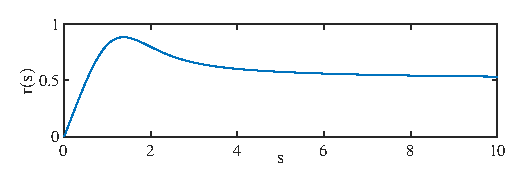
\includegraphics[scale=1.4]{figures/MFG-information}
	\caption{The graph of $r(s) = \frac{2s\left(c(S)\partial_{11}c(S) - (\partial_1c(S))^2\right)}{c(s)\left(c(S)-\partial_{11}c(S)\right)}$ against $s$. \label{fig:MFG-information}}
\end{figure}

The proposed closed form solution of MLE is essential for designing and implementing recursive stochastic filters based on MFG, as it is inevitably used in each step of uncertainty propagation and measurement update, which typically run at more than $\SI{100}{\hertz}$.
It is not feasible to solve the joint MLE numerically at every step for real-time implementations.
